\begin{event}{OpenDreamKit annual meeting}{2016-06-27-bremen}{Bremen (Germany) 2016-06-27 to 2016-07-01}{PS,LL,SA,JU,UW,USH,UV,ZH,USO,US,SR}{24}{http://opendreamkit.org/meetings/2016-06-27-Bremen/}

  \textbf{Main goals.} Annual project meeting meeting, informal review and workshops

  \textbf{ODK implication.} JacobsUni (Bremen) hosted this event which
  was coorganized by Paris Sud and fully funded by ODK.

  \textbf{Event summary.} The beginning of the week was dedicated to
  ODK’s open and internal meetings, including an informal review with
  our Project Officer and three EU Commission reviewers. The rest of
  the week was dedicated to joint work sessions on WP4 (User
  Interfaces) and WP6 (Data/Knowledge/Software bases, aka
  Math-in-the-middle) activities.

  \textbf{Demographic.} 21 ODK participants together with ODK's
  project officer and three reviewers from the EU Commission.

  \textbf{Results and impact.} This meeting was the occasion to build
  a common overview of what was achieved during the first ten months,
  and plan together work on the upcoming tasks and deliverables. The
  informal project review was enormously helpful to get early feedback
  and start preparing for the upcoming formal review at Month 18
  (March 2017).


  % \begin{figure}[ht]
  %   \caption*{ODK Kickoff meeting}
  %   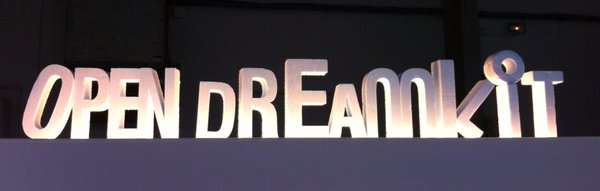
\includegraphics[scale=0.3]{pictures/kickoff1.jpg}
  % \end{figure}
\end{event}
